\chapter{DCViz: Visualization of Data}

With an increasingly massive code framework comes the increased need of data analysis tools. Data analysis usually involves visualization of the data; there is only so much information a single number can hold. To supplement the QMC code, a visualization tool has been developed.

The tool DCViz (Dynamic Column data Visualizer) is a Python based visualization tool designed to plot data stored in columns. The plot library used is \textit{Matplotlib}. The data can be plotted dynamically at a specified interval, and is hence designed to run parallel to the main application, e.g. DMC. The convergence of the DMC method is much better represented by a trailing energy graph than simply a stream of numbers. The same goes for the minimization process.

\section{Basic Usage}

Just like for the \verb+orbitalsGenerator+ tool (see Appendix \ref{appendix:sympy}), specific implementations come in the shape of subclasses of the DCViz superclass. All the functionality regarding setting up figures, re-plotting dynamically, clearing figures to avoid random crashes if used repeatedly, etc. is inherited from the superclass. The necessary elements to implement is

\begin{small}
\begin{tabular}{lp{12cm}}
\verb+figMap+		& A dictionary representing the names and structure of the plotted figures. \\						& \verb+figMap = {"fig1": ["subFig1", "subFig2", "subFig3"], "fig2": ["subFig4"]}+ \\
			& Will create two figures, where the first is split into three sub-figures.\\
			& In class member functions, \verb+self.subFig1+ will be available as the figure representing the first sub-figure of \verb+self.fig1+. \\
			\ \\
\verb+nametag+		& A string, e.g. \verb|nametag = "DMC_out_\d+\.dat"|, representing the name of the output files 				associated with the given implementation (subclass). Full regular expressions support. Used in 				order to automatically detect which subclass to load for a specific file.\\
			\ \\
\verb+plot(self, data)+& The loaded file will be loaded into a \verb+data+ object, which is an iterator where each elements
			represents a column in the data file. Designed such that expressions like \verb+col1, col2 = data+ is possible (and fast). To access the raw data as a matrix, use \verb+data.data+ \\
			\ \\
			&In the plot function, the sub-figures introduced in \verb+figMap+ should be loaded with data through e.g. \verb+self.subFig1.plot(col1, col2)+. 
\end{tabular}
\end{small}

An example implementation would be

\vspace{0.5cm}
\begin{lstlisting}[language=Python]
#DCViz_classes.py

from DCViz_sup import DCVizPlotter

class myTestClass(DCVizPlotter):
    nametag =  'testcase\d\.dat' #filename with regex support
    
    #1 figure with 1 subfigure
    figMap = {'fig1': ['subfig1']}
    
    #skip first row.
    skipRows = 1    
    
    def plot(self, data):
        column1 = data[0]

        self.subfig1.set_title('I have $\LaTeX$ support!')
              
        self.subfig1.set_ylim([-1,1])
          
        self.subfig1.plot(column1)
\end{lstlisting}



\subsubsection{Additional Support}

Additional parameters can be overloaded for additional functionality

\begin{small}
\begin{tabular}{lp{14cm}}
\verb+nCols+ & The number of columns present in the file. Will be automatically detected unless the data is stored in binary format.\\
\verb+skipRows+ & The number of initial rows to skip. Will be automatically detected unless the data is stores as a single column.\\
\verb+skipCols+ & The number of initial columns to skip. Defaults to zero.\\
\verb+armaBin+ & Boolean flag. If set to true, the data is assumed to be stored in Armadillo's binary format (doubles). Number of columns and rows will be read from the file header.\\
\verb+fileBin+ & Boolean flag. If set to true, the data is assumed to be stores in binary format. The number of columns must be specified.
\end{tabular}
\end{small}

The \LaTeX support is enabled if the correct packages is installed.

\subsubsection{Families}

A specific implementation can be flagged to belong to a family by setting the class member variable \verb+isFamilyMember+ to true. If this flag is true, the folder where the originally data was loaded will be scanned for additional matches, all of which will be loaded into the \verb+data+ input to the plot function. In this case each element of the \verb+data+ list would be a column iterator as explained previously.

To keep track of which file a given data-set was loaded from, a list \verb+self.familyFileNames+ is created, where element $i$ is the filename corresponding to \verb+data[i]+.

A class member string \verb+familyName+ can be overridden to display a more general name in the auto-detection feedback. An example implementation using data file families would be
\vspace{0.5cm}
\begin{lstlisting}[language=Python]
#DCViz_classes.py

from DCViz_sup import DCVizPlotter

class myTestClassFamily(DCVizPlotter):
    nametag =  'testcaseFamily\d\.dat' #filename with regex support
    
    #1 figure with 3 subfigures
    figMap = {'fig1': ['subfig1', 'subfig2', 'subfig3']}
    
    #skip first row of each data file.
    skipRows = 1    

    #Using this flag will read all the files matching the nametag
    #(in the same folder.) and make them aviable in the data arg    
    isFamilyMember = True
    familyName = "testcase"
    
    def plot(self, data):
        
        #figures[0] is 'fig1' figures. the 0'th element is the
        #self.fig1 itself. Subfigures are always index [1:]
        mainFig = self.figures[0][0]  
        mainFig.suptitle('I have $\LaTeX$ support!')        
        subfigs = self.figures[0][1:]
    
        #Notice we plot fileData.data (In order to get the numpy object) 
        #and not fileData alone, as fileData is a 'dataGenerator' instance 
        #used to speed up file reading. Alternatively, we could send data[:]
        for subfig, fileData in zip(subfigs, data):
            subfig.plot(fileData.data)
            subfig.set_ylim([-1,1])
\end{lstlisting}

loading e.g. \verb+testcaseFamily0.dat+ would automatically load \verb+testcaseFamily1.dat+ etc. as well.


\subsubsection{The Application Programming Interface (API)}

The DCViz library has been developed to interface nicely with any Python script \footnote{DCViz can also be called through C++, however, no header has been implemented for this. Typically one would use the std::system or std::thread to start the script in the background.}. Given a path to the data file, all that is needed in order to visualize it is

\vspace{0.5cm}
\begin{lstlisting}[language=Python]
import DCVizWrapper as viz
dynamicMode = False #or true

...
#Perform some calculations and store these in the file myDataFile (including path)

#DCVizWrapper.main() automatically detects the subclass implementation 
#matching the specified file. Thread safe and easily interruptable.
viz.main(path=myDataFile, dynamic=dynamicMode)
\end{lstlisting}

\subsubsection{The Terminal Client}

The \verb+DCVizWrapper.py+ script can also be called directly from a terminal using the path as first command line argument. If the option \verb+-d+ is supplied, dynamic mode is activated.

\subsubsection{The GUI}

The script \verb+DCVizGUI.py+ sets up a GUI for visualizing data using DCViz. The GUI is implemented using pyside (python wrapper for Qt), and is designed to be simple. Data files are loaded from an open-file dialog, and will appear in a drop-down menu once loaded. The play button executes the main loop of the currently selected data file. Dynamic mode is selected though a check-box, and the refresh interval is set by a slider (from zero to ten seconds). Warnings can be disabled through the configuration file.

The GUI can be opened from any Python script by calling the \verb+main+ function (should be threaded if used as part of another application). If a path is supplied to the function,
this path will be default in all file dialogues. Defaults to the current working directory.

The following is a tiny script executing the GUI for a QMC application. If no path is supplied at the command line,
the default path is set to the scratch path.

\vspace{0.5cm}
\begin{lstlisting}[language=Python]
import sys, os
from pyLibQMC import paths #contains all files specific to the QMC library

#Adds DCVizGUI to the Python path
sys.path.append(os.path.join(paths.toolsPath, "DCViz", "GUI"))

import DCVizGUI

if __name__ == "__main__":

    if len(sys.argv) > 1:
        path = sys.argv[1]
    path = paths.scratchPath
   
    sys.exit(DCVizGUI.main(path))
\end{lstlisting}

Alternatively, \verb+DCVizGUI.py+ can be executed directly from the terminal with an optional default path as first command line argument. 

The following is the terminal feedback supplied from opening the GUI

\begin{verbatim}
 ~/.../DCViz/GUI$ python DCVizGUI.py
[ Detector ]:  Found subclasses 'myTestClass', 'myTestClassFamily', 'EnergyTrail', 
'Blocking', 'DMC_OUT', 'radial_out', 'dist_out', 'testBinFile', 'MIN_OUT'
[   GUI    ]:  Data reset.
\end{verbatim}

Selecting a folder from the open-folder dialog initializes the detector on all file content

\begin{verbatim}
[ Detector ]:  matched [  DMC_out.dat  ] with [    DMC_OUT    ]
[ Detector ]:  matched [  ASGD_out.dat ] with [    MIN_OUT    ]
[ Detector ]:  matched [blocking_DMC_out.dat] with [    Blocking   ]
[ Detector ]:  'blocking_MIN_out0_RAWDATA.arma' does not match any DCViz class
[ Detector ]:  'blocking_DMC_out_RAWDATA.arma' does not match any DCViz class
[ Detector ]:  matched [blocking_VMC_out.dat] with [    Blocking   ]
\end{verbatim}

All matched files will be listed in the drop-down menu. Selecting a file, and pressing the play button initializes a job. Pressing the stop button (replacing the play in case of dynamic mode), will end the job. All jobs are threaded, hence several non-dynamic jobs can be ran at once. The limit is set to one dynamic job pr. application. 

\begin{verbatim}
[   Job    ]:  Starting.
[   Job    ]:  Stoping...  Stopped.
\end{verbatim}

Screen-shots of the GUI taken in the process listed previously is given in Fig. \ref{fig:gui}.

\begin{figure}
 \begin{center}
  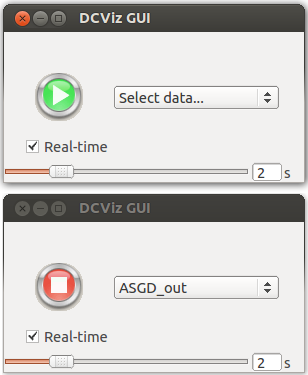
\includegraphics{../Graphics/gui.png}
  \caption{Two consequent screen shots of the GUI. The first (top) is taken directly after the detector is finished loading files into the drop-down menu. The second is taken directly after the job is started.}
  \label{fig:gui}
 \end{center}
\end{figure}

The terminal tracker can be silenced through to configuration file to not interfere with the standard output of an application. Alternatively, the GUI thread can redirect its standard output to file.





